\subsection{Modality transfer with CNN}

\label{sec:modality_transfer}

\begin{frame}{Modality Hallucination Network}
	\begin{block}{Original contribution}
		From \cite{Hoffman2016}, applied for the task of semantic interpretation with Fast-RCNN.
	\end{block}
	\vfill	
	\begin{minipage}[c]{0.49\linewidth}
		\begin{block}{Modality hallucination training}
			\includegraphics[width=0.9\linewidth]{vect/hallucination.pdf}					
		\end{block}
	\end{minipage}
	\begin{minipage}[c]{0.49\linewidth}
		\begin{block}{The network at test time}
			\includegraphics[width=0.9\linewidth]{vect/hallucination_testing.pdf}	
		\end{block}
	\end{minipage}
\end{frame}

\begin{frame}{Depth map inference}	
	\includegraphics[width=\linewidth]{images/kusnietzov.png}				
	
	\cite{Kuznietsov2017}
	
	CNN can learn a model to transform a input from one modality to another (widely used to infer depth map from monocular images).
	\vfill
	\begin{block}{Intuition}
		As we already use a neural network to describe our data, we should use this kind of architecture to transfer the knowledge among modalities during training.
	\end{block}	 	
	
\end{frame}

\begin{frame}{Proposed architecture}	
	\begin{minipage}[c]{0.48\linewidth}
		\begin{block}{Encoder-Decoder architecture}
			\includegraphics[width=\linewidth]{vect/encoderdecoder.pdf}					
		\end{block}
	\end{minipage}
	\hfill
	\begin{minipage}[c]{0.48\linewidth}
		\begin{block}{Encoder-Decoder training scheme}
			\includegraphics[width=\linewidth]{vect/encoderdecoder_training.pdf}	
		\end{block}
	\end{minipage}
	\vfill
	Decoder part is initialized with pre-trained weights and decoder network is randomly initialized.				
\end{frame}